%! TEX root = **/010-main.tex
% vim: spell spelllang=en:

\section{Results}

\subsection{Replicating results from Kutznetsov et al.}

To analyze the performance of the program the system found by Kutznetsov et al.
\cite{kuznetsov_visualization_2013} will be used.
\footnote{This system is the same that was previously discussed
in~\cref{sec:context} (\cref{fig:kuznetsov})}

\Cref{eq:kuznetsov} shows the system and its parameters and \cref{fig:kuznetsov2}
shows the limit cycles.

\begin{equation}%
    \label{eq:kuznetsov}
    \begin{split}
        \frac{dx}{dt} &= x^2 + xy + y^2 + x + y\\
        \frac{dy}{dt} &= ax^2 + bxy * cy^2 + \alpha x \beta y
    \end{split}
    \qquad \qquad
    \begin{split}
        a &= -10\\
        b &= 2.2\\
        c &= 0.7\\
        \alpha &= -72.7778\\
        \beta &= 0.0015
    \end{split}
\end{equation}

\begin{figure}[H]
    \centering
    \includegraphics[width=1.0\textwidth]{4cycles}
    \caption{Visualization of four limit cycles in two-dimensional polynomial quadratic system, from Ref.~\cite{kuznetsov_visualization_2013}
    }%
    \label{fig:kuznetsov2}
\end{figure}

\Cref{fig:kuznetsov_cuda} shows a visualization of the points which a ratio
equal to one with tolerance $10^{-6}$. These correspond exactly with the results
of~\cite{kuznetsov_visualization_2013}. The computation of this data took 250ms
and using a grid of $1024 \times 1024$ trajectories, and a fixed \emph{Runge Kutta}
of third order with a step size of $10^{-3}$. Notice that some points left of $x
= 0$ are not found. Nevertheless, the cycles can be identified easily.

\begin{figure}[H]
    \centering
    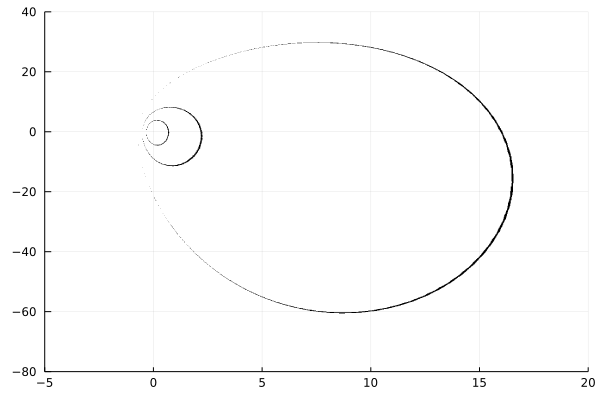
\includegraphics[width=1.0\textwidth]{kutznetsov_cuda}
    \caption{Limit cycles found using our program ($1024^2$ grid)}%
    \label{fig:kuznetsov_cuda}
\end{figure}

Using a bigger grid size of $5000\times5000$, we obtain clearer results but it takes
1200ms. There is not much benefit in this instance since the cycles are clear and
we are searching inside a well delimited plane, but when the search space is greater
it does offer a benefit.

\begin{figure}[H]
    \centering
    \includegraphics[width=1.0\textwidth]{kutznetsov_cuda_5k}
    \caption{Limit cycles found using our program ($5000^2$ grid)\\
        Black areas correspond to points from which trajectories have
        a rate of 1 (tol $10^{-6}$)
    }%
    \label{fig:kuznetsov_cuda_5k}
\end{figure}

\begin{figure}[H]
    \centering
    \includegraphics[width=1.0\textwidth]{histograms}
    \caption{Histogram of distribution of values for each local extrema with rate of change
        equal to 1 (tol $1^{-6}$).
    }%
    \label{fig:histograms}
\end{figure}

If we apply \emph{Kmeans} clustering on the result
